\documentclass[11pt]{article}

%%%%%%%%%%%%%%Include Packages%%%%%%%%%%%%%%%%%%%%%%%%%%
\usepackage{xcolor}
\usepackage{mathtools}
\usepackage[a4paper, total={6in, 8in}, margin=1.25in]{geometry}
\usepackage{amsmath}
\usepackage{amssymb}
\usepackage{paralist}
\usepackage{rsfso}
\usepackage{amsthm}
\usepackage{wasysym}
\usepackage[inline]{enumitem}   
\usepackage{hyperref}
\usepackage{tocloft}
\usepackage{titlesec}
\usepackage{colortbl}
\usepackage{wrapfig}
\usepackage{pdfpages}
\usepackage[american]{circuitikz}
%%%%%%%%%%%%%%%%%%%%%%%%%%%%%%%%%%%%%%%%%%%%%%%%%%%%%%%%



\begin{document}
\Large \noindent \textbf{Physics 5C Discussion (Week 9)}\\
\normalsize
Department of Physics and Astronomy, UCLA\\
%\noindent TA: Jinyan Miao (jnmiu@ucla.edu)\\
%Office hours: Thursday 10-11 AM $\&$ 1-2 PM at PAB 2-429\\
%Tutoring center hours: Friday 2-3 PM at PAB 2-429 (Zoom room also available)\\
\noindent\rule{8cm}{0.4pt}\\
\textbf{Problem 1}:
Jinyan is trying to determine the work function (binding energy) $\phi$ of a mysterious metallic material. He uses two different lasers to shine two different monochromatic lights on the metal. The first laser that he uses is a helium-neon laser, which produces a red light with wavelength $\lambda_{r}=633\,$nm. The second laser is a nitrogen laser, which produces an ultraviolet light with wavelength $\lambda_u = 337\,$nm. The helium-neon laser is very powerful, and it can deliver $1919\,$J of energy per second onto the surface of the mysterious metal. The nitrogen laser is much weaker, and it can deliver only around $19$\,J of energy per second onto the surface of the metal. \\

\noindent\textbf{Part (a)} Find the frequencies of the lights emitted by the two lasers.\\

\noindent\textbf{Part (b)} Find the energy of the photons emitted by the lasers, in both eV and J. \\

\noindent\textbf{Part (c)} If it is found that the electrons on the metal surface are ejected with a kinetic energy $\text{KE}\approx 0$\,eV when the nitrogen laser is used, what will be the maximal kinetic energy of those ejected electrons (if any) if the helium-neon laser is used?\\

\noindent\textbf{Part (d)} If it is found instead that the electrons on the metal surface are ejected with a kinetic energy $\text{KE}\approx 0$\,eV when the helium-neon laser is used, what will be the maximal kinetic energy of those ejected electrons (if any) if the nitrogen laser is used?\\

\noindent\textbf{Part (e)} Based on part (d), find the de Broglie wavelength of the electron that has its maximal kinetic energy, ejected by the nitrogen laser.


\newpage
\begin{wrapfigure}[5]{r}{0.45\textwidth}
  \begin{center}
  \vspace{-10pt}
    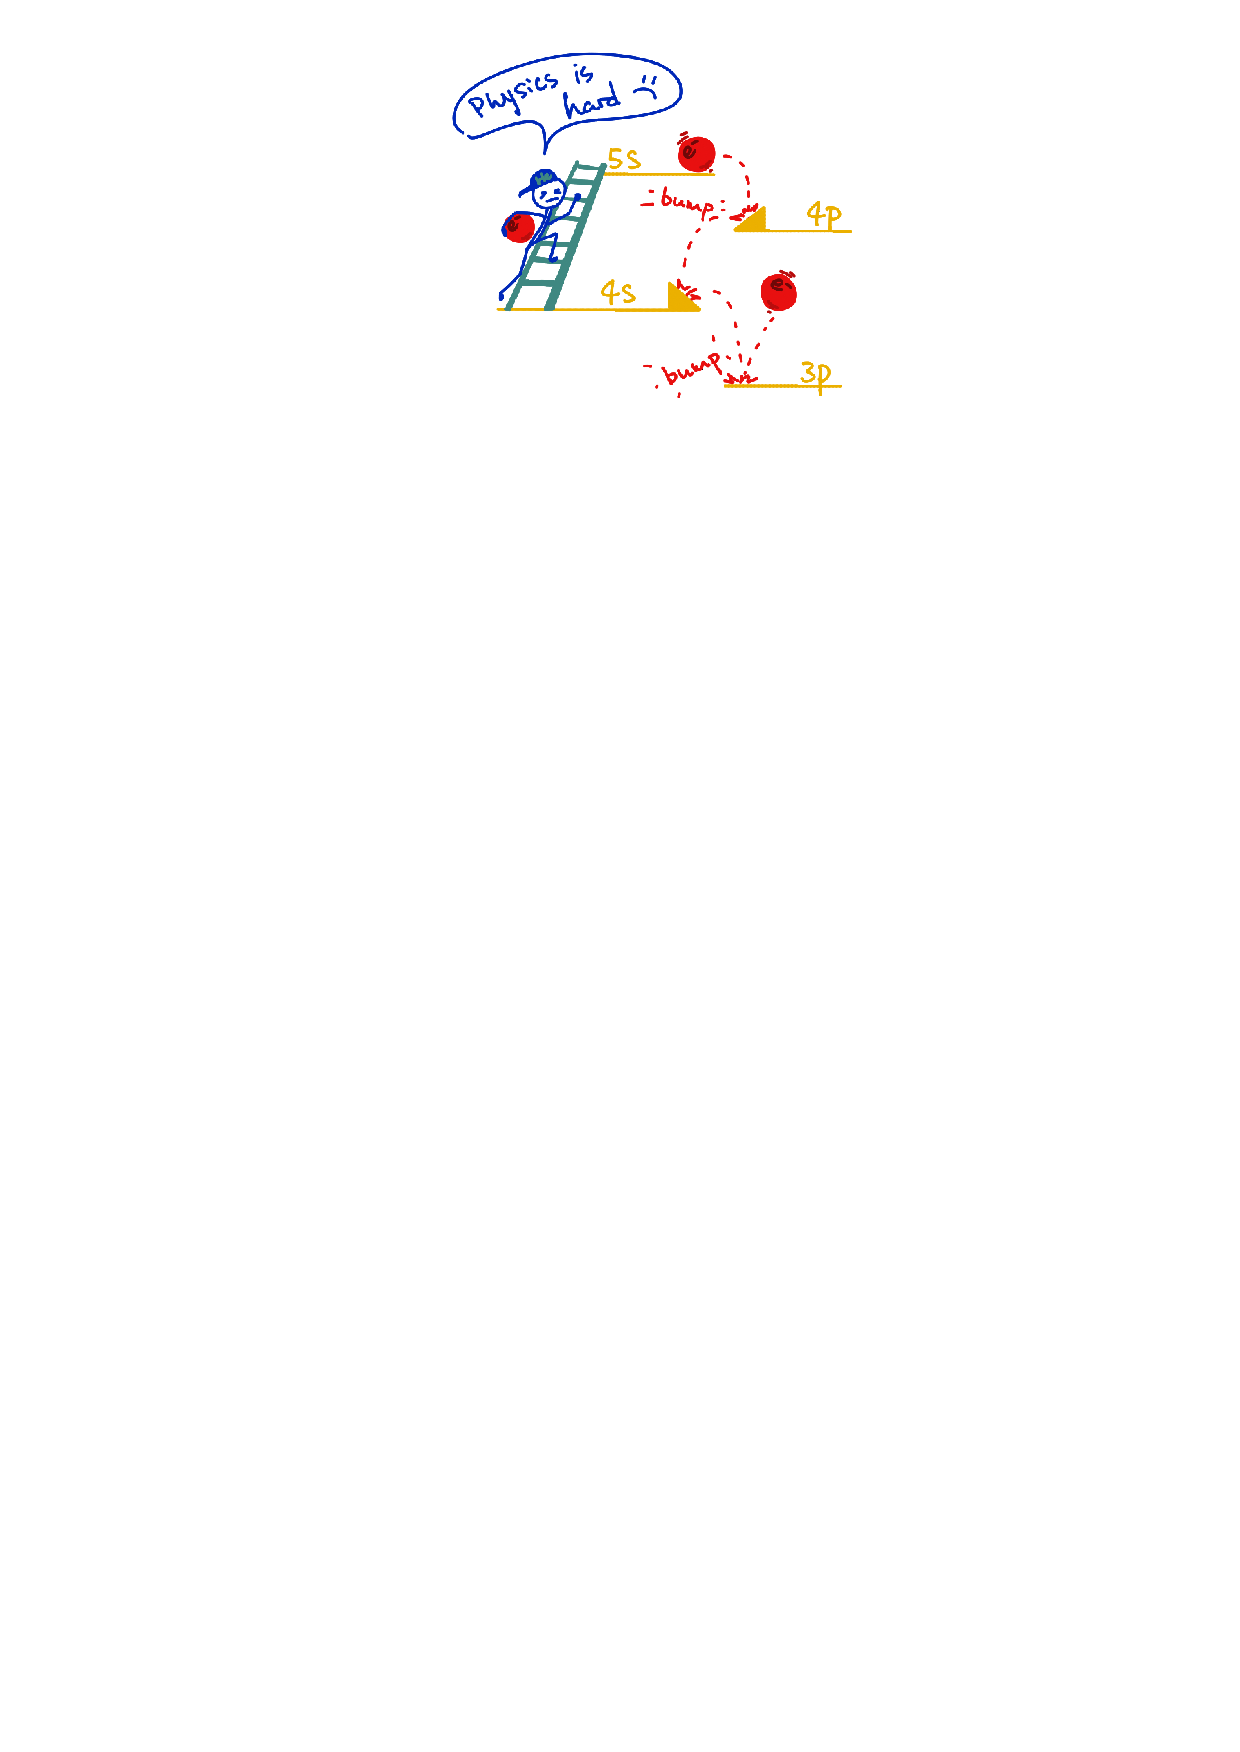
\includegraphics[scale=0.85]{heliumNeon}
  \end{center}
\end{wrapfigure}
\noindent\textbf{Problem 2}:
The energy that the electrons surrounding a neon nucleus could have is quantized - only some discretized values are allowed. Here are some of the energy levels that the electrons in a neon atom could have:
\begin{enumerate}
\item The ``3p" state energy level is $18.70$\,eV.
\item The ``4s" state energy level is $19.78$\,eV.
\item The ``4p" state energy level is $20.30$\,eV.
\item The ``5s" state energy level is $20.66$\,eV.
\end{enumerate}
An atomic energy-level transition corresponds to an electron jumping from one of those energy levels to another, but this process requires emitting (if jumping from high to low energy level) or absorbing (if jumping from low to high energy level) a photon to ensure energy conservation. The operation of a laser is based on quantum mechanics: It makes use of atomic transitions to emit the photon with the correct wavelength. For the helium-neon laser, the emitted red light is mainly from an atomic transition in neon.\\

\noindent\textbf{Part (a)} Based on the information given, the production of the red light is based on an atomic transition between which two of the listed energy levels? \footnote{Hint: The ``jump" does not have to be between consecutive states. That is, an electron is allowed to jump from the 4p state to the 3p state by emitting a photon.} \footnote{Another Hint: This part requires no more than a single subtraction of numbers. Part (b) of Problem 1 will also be helpful.}\\

\noindent\textbf{Part (b)} The role of helium in the helium-neon laser is to ``pump" electrons in the neon atom from state 4s to state 5s. Find the wavelength of the photon absorbed by the electron in the neon atom in this process.


\newpage
\section*{Problem 1}
The key idea in this problem is that the energy of a single photon depends only on the light frequency (or wavelength), not on how powerful the laser is overall. A more powerful laser just sends more photons per second, but it does not make each individual photon more energetic. For the photoelectric effect, the important equation is
\begin{align*}
\text{KE}_{\max} = hf - \phi\,,
\end{align*}
where $h$ is Planck's constant and $\phi$ is the work function of the metal. We will use
\begin{align*}
h = 6.63\times 10^{-34}\,\text{J}\cdot \text{s}\,,\qquad
c=3.0\times 10^8\,\text{m/s}\,,\qquad
1\,\text{eV}=1.6\times 10^{-19}\,\text{J}\,.
\end{align*}

\noindent\textbf{Part (a)} The frequency of light is related to the wavelength by
\begin{align*}
f = \frac{c}{\lambda}\,.
\end{align*}
For the red helium-neon laser,
\begin{align*}
f_r = \frac{3.0\times 10^8\,\text{m/s}}{633\times 10^{-9}\,\text{m}}
= 4.74\times 10^{14}\,\text{Hz}\,.
\end{align*}
For the ultraviolet nitrogen laser,
\begin{align*}
f_u = \frac{3.0\times 10^8\,\text{m/s}}{337\times 10^{-9}\,\text{m}}
= 8.90\times 10^{14}\,\text{Hz}\,.
\end{align*}

\noindent\textbf{Part (b)} The energy of one photon is
\begin{align*}
E = hf\,.
\end{align*}
For the red photon,
\begin{align*}
E_r &= (6.63\times 10^{-34})(4.74\times 10^{14})\,\text{J}\\
&= 3.14\times 10^{-19}\,\text{J}\,.
\end{align*}
Converting this to eV,
\begin{align*}
E_r = \frac{3.14\times 10^{-19}\,\text{J}}{1.6\times 10^{-19}\,\text{J/eV}}
= 1.96\,\text{eV}\,.
\end{align*}

For the ultraviolet photon,
\begin{align*}
E_u &= (6.63\times 10^{-34})(8.90\times 10^{14})\,\text{J}\\
&= 5.90\times 10^{-19}\,\text{J}\,,
\end{align*}
so in eV,
\begin{align*}
E_u = \frac{5.90\times 10^{-19}\,\text{J}}{1.6\times 10^{-19}\,\text{J/eV}}
= 3.69\,\text{eV}\,.
\end{align*}
Therefore,
\begin{align*}
E_r = 1.96\,\text{eV} = 3.14\times 10^{-19}\,\text{J}\,,\qquad\qquad
E_u = 3.69\,\text{eV} = 5.90\times 10^{-19}\,\text{J}\,.
\end{align*}

\noindent\textbf{Part (c)} If the nitrogen laser ejects electrons with $\text{KE}\approx 0$\,eV, then the ultraviolet photons are just barely able to free the electrons. That means the work function of the metal must be
\begin{align*}
\phi \approx E_u = 3.69\,\text{eV}\,,
\end{align*}
because $\text{KE}_{\max} \approx 0 = E_u- \phi$. Now compare this with the energy of a red photon:
\begin{align*}
E_r = 1.96\,\text{eV} < \phi = 3.69\,\text{eV}\,.
\end{align*}
So a red photon does not even have enough energy to overcome the work function. Therefore \underline{no electrons are ejected at all} by the helium-neon laser, and hence there is no maximal kinetic energy to compute.\\

This is the important physics point: Even though the helium-neon laser is much more powerful overall, each red photon still has too little energy to eject an electron from this metal. Whether or not an electron can be ejected from the metal does not depend on how ``powerful" the laser is. It only depends on how ``powerful" each photon is. This is a straightforward comparison between the wave nature (laser power) and particle nature (photon energy) of light.\\

\noindent\textbf{Part (d)} Now suppose instead that the helium-neon laser ejects electrons with $\text{KE}\approx 0$\,eV. Then the red photons are just at the threshold, so the work function must be
\begin{align*}
\phi \approx E_r = 1.96\,\text{eV}\,,
\end{align*}
because $\text{KE}_{\max} \approx 0 =E_r - \phi$. For the nitrogen laser, the maximal kinetic energy is then
\begin{align*}
\text{KE}_{\max} = E_u - \phi = 3.69\,\text{eV} - 1.96\,\text{eV} = 1.73\,\text{eV}\,.
\end{align*}
Converting this to Joules,
\begin{align*}
\text{KE}_{\max} = (1.73)(1.6\times 10^{-19})\,\text{J}
= 2.77\times 10^{-19}\,\text{J}\,.
\end{align*}
So the maximal kinetic energy of the ejected electrons is
\begin{align*}
\text{KE}_{\max} = 1.73\,\text{eV} = 2.77\times 10^{-19}\,\text{J}\,.
\end{align*}

\noindent\textbf{Part (e)} The de Broglie wavelength is
\begin{align*}
\lambda = \frac{h}{mv}\,.
\end{align*}
To find the momentum $mv$ of the electron, we use the non-relativistic kinetic energy formula for electron with mass $m_e$, 
\begin{align*}
\text{KE} = \frac{1}{2}m_ev^2\,,
\end{align*}
so the momentum $m_ev$ of the electron is
\begin{align*}
m_ev = \sqrt{2m_e\text{KE}}\,.
\end{align*}
The kinetic energy is the one we found in part (c) and the mass is the electron mass,
\begin{align*}
\text{KE} = 2.77\times 10^{-19}\,\text{J}\,,\qquad
m_e = 9.11\times 10^{-31}\,\text{kg}\,.
\end{align*}
Therefore, we find the momentum of the electron to be
\begin{align*}
m_ev = 7.10\times 10^{-25}\,\text{kg}\cdot\text{m/s}\,.
\end{align*}
Now plug this into the de Broglie formula to get the de Broglie wavelength of electron,
\begin{align*}
\lambda = \frac{h}{m_ev}=\frac{6.63\times 10^{-34}}{7.10\times 10^{-25}}\,\text{m}
= 9.34\times 10^{-10}\,\text{m}= 0.93\,\text{nm}\,.
\end{align*}


\section*{Problem 2}
In this problem, each atomic transition corresponds to an energy difference between two allowed energy levels. If the atom emits a photon, then the emitted photon energy must equal the energy difference between the higher state and the lower state. If the atom absorbs a photon, then the absorbed photon energy must equal the energy needed to jump upward.\\

\noindent\textbf{Part (a)} From Problem 1, the red helium-neon laser has wavelength $\lambda_r = 633\,$nm, so its photon energy is about
\begin{align*}
E_r = 1.96\,\text{eV}
\end{align*}
as we have calculated in part (b) of Problem 1. Now we compare this with the differences between the listed neon energy levels. The difference between the 5s and 3p levels is
\begin{align*}
20.66\,\text{eV} - 18.70\,\text{eV} = 1.96\,\text{eV}\,.
\end{align*}
This matches the red photon energy. Therefore the red light is produced by the transition
\begin{align*}
\text{5s} \longrightarrow \text{3p}\,.
\end{align*}
Since this is an emission process, the electron jumps from the higher-energy 5s state down to the lower-energy 3p state, and the energy difference comes out as a photon.\\

\noindent\textbf{Part (b)} Now the electron is being pumped from 4s to 5s, so it must \underline{absorb} a photon whose energy equals the difference between those two levels:
\begin{align*}
\Delta E = 20.66\,\text{eV} - 19.78\,\text{eV} = 0.88\,\text{eV}\,.
\end{align*}
We combine $c=\lambda f$ and $E = hf$ to get
\begin{align*}
E =hf =  \frac{hc}{\lambda}\,.
\end{align*}
An easy way to do this in eV is to use $hc \approx 1240\,\text{eV}\cdot\text{nm}\,.$ Therefore the required absorbed wavelength is
\begin{align*}
\lambda = \frac{hc}{E}=\frac{1240\,\text{eV}\cdot\text{nm}}{0.88\,\text{eV}}
= 1.41\times 10^3\,\text{nm} = 1.41 \cdot 10^{-6}\,\text{m}\,.
\end{align*}
Please make sure to use the quantities in the correct units. That is, if you prefer to write everything in eV, do all calculation in eV. If you prefer to write everything in Joules, do all calculation in Joules. 

\vfill

\begin{center}

\includegraphics[scale=0.135]{michgiganLake}\\
\hfill\break
Another sunrise at Lake Michigan at Chicago, IL. Pictured in March 2026.\\
\end{center}



\end{document}
